\menudef{menu.help.manual}

The application's manual is available as either a \gls{pdf}
document, which can be viewed outside of the application, or as a
set of \gls{html} files which can be viewed within the application
via the \menu{help.manual} menu item. This will open the primary
help window (\sectionref{sec:primaryhelp}), but some dialog boxes
may also have a \inlineglsdef{action.help} button that will open a secondary help
dialog (\sectionref{sec:secondaryhelp}).

Both the primary help window and the secondary help dialog windows
have a panel that shows a page of the manual (a
\inlineglsdef{index.help-page}).  Note that \qt{page} in this
context refers to the \gls{html} file displayed in the help window, which
typically contains a section, and doesn't relate to the page numbers
in the \gls{pdf}. The \gls{html} index page is obtained from the
same source code as the \gls{pdf} index page, but the locations are
converted from a \gls{pdf} page number to the \gls{html} page title
(preceded by the marker \gls{symbol.location_prefix}).

\menudef{index.menu.helppage}

The \gls{index.menu.helppage} (see \figureref{fig:helppagepopup})
can be activated on the current \dgls{help-page} for both the primary and
secondary help windows. The menu has the following items.

\FloatSubFigs
{fig:helppagepopup}
 {
   {fig:helpframepopup}
   {\includeimg
     [alt=
      {Primary help window popup menu}
     ]{images/helppagepopup}%
   }
   {Primary},
   {fig:helpdialogpopup}
   {\includeimg
     [alt=
      {Secondary help multi-page dialog popup menu}
     ]{images/helpdialogpopup}%
   }
   {Secondary (Multi)},
   {fig:helpdialogsinglepopup}
   {\includeimg
     [alt=
      {Secondary help single-page dialog popup menu}
     ]{images/helpdialogsinglepopup}%
   }
   {Secondary (Single)}
}
[Help Page Popup Menus]
{Help Page Popup Menus: 
 \subfigref{fig:helpframepopup} Primary Help Window;
 \subfigref{fig:helpdialogpopup} Secondary Help Dialog
 with Multiple Topic Pages;
 \subfigref{fig:helpdialogsinglepopup} Secondary Help Dialog
 with Single Topic Pages}

\menudef{menu.helppage.view_image}

If the popup menu is activated over an image, the \menu{helppage.view_image}
item will open the \dialog{imageviewer} window (see
\sectionref{sec:helpimageviewer}) which can be used to enlarge the
image. This item will be disabled if the popup menu wasn't activated
over an image.

\menudef{menu.helppage.home}

If the popup menu is activated on the primary help window
(\figureref{fig:helpframepopup}), this will
behave as the \menu{helpframe.navigation.home} menu item (which
switches the current page to the first page of the document).
This menu item is not available on secondary help windows.

\menudef{menu.helppage.reset}

If the popup menu is activated on the secondary help dialog
(\figuresref{fig:helpdialogpopup,fig:helpdialogsinglepopup}), this
will behave as the \menu{helpdialog.navigation.reset} menu item
(which switches the current page back to the relevant page or the
first in the applicable section of the dialog topic).
This menu item is not available on the primary help window.

\menudef{menu.helppage.up}

If the popup menu is activated on the primary help window or on the
secondary help window that has multiple pages, then this will behave
as the primary \menu{helpframe.navigation.up} or
secondary \menu{helpdialog.navigation.up} menu items. (That is, it
will move up a hierarchical level, if available.)

\menudef{menu.helppage.previous}

If the popup menu is activated on the primary help window or on the
secondary help window that has multiple pages, then this will behave
as the primary \menu{helpframe.navigation.previous} or
secondary \menu{helpdialog.navigation.previous} menu items.
(That is, it will move to the previous page, if available.)

\menudef{menu.helppage.next}

If the popup menu is activated on the primary help window or on the
secondary help window that has multiple pages, then this will behave
as the primary \menu{helpframe.navigation.next} or
secondary \menu{helpdialog.navigation.next} menu items.
(That is, it will move to the next page, if available.)

\menudef{menu.helppage.historyback}

This will behave as the primary
\menu{helpframe.navigation.historyback} or secondary
\menu{helpdialog.navigation.historyback} menu items.
(That is, it will move back a page in the history list, if available.)

\menudef{menu.helppage.historyforward}

This will behave as the primary
\menu{helpframe.navigation.historyforward} or secondary
\menu{helpdialog.navigation.historyforward} menu items.
(That is, it will move forward a page in the history list, if available.)


\section{The Primary Help Window}
\label{sec:primaryhelp}

The main help frame has a panel that shows a page of the manual (a
\dgls{help-page}). Links in the page and the \gls{gui} navigation
elements provide a way to switch to a different page.

There is a menu bar with items for navigation actions or adjusting
\gls{gui} settings. Some menu items are replicated as buttons in the
toolbar, which is split into different regions: navigation, lookup,
settings, and history. The forward, up and next navigation actions
can also be implemented by buttons in the lower navigation panel at
the bottom of the window.

\menudef*{menu.helpframe.navigation}

The \menu{helpframe.navigation} menu provides a way to move around
the document.
\Figureref{fig:navbuttons} shows the corresponding four navigation
buttons in the toolbar: \btn{helpframe.navigation.home} (go to the
start of the manual), \btn{helpframe.navigation.previous} (go to the
previous section), \btn{helpframe.navigation.up} (go to parent
section), and \btn{helpframe.navigation.next} (go to the next
section).

\FloatFig
{fig:navbuttons}
{\includeimg
 [alt=
   {
     [\entrytooltip{menu.helpframe.navigation.home} Button]
     [\entrytooltip{menu.helpframe.navigation.previous} Button]
     [\entrytooltip{menu.helpframe.navigation.up} Button]
     [\entrytooltip{menu.helpframe.navigation.next} Button]
   }
 ]{images/navbuttons}%
}
[Navigation Buttons]{Navigation Buttons (Home, Previous, Up, Next)}

\menudef{menu.helpframe.navigation.home}

The \menu{helpframe.navigation.home} item, which is also available
as a button on the toolbar, will replace the current view with the
first page of the document.

\menudef{menu.helpframe.navigation.up}

The \menu{helpframe.navigation.up} item, which is also available
as a button on the toolbar, will replace the current view with the
parent page of the current hierarchical level. The item and button
will be disabled if there is no parent page (that is, if the current
page is the document's home page). The parent page may
also be the previous page if the current page is the first in its
current hierarchical level.

\menudef{menu.helpframe.navigation.previous}

The \menu{helpframe.navigation.previous} item, which is also available as
a button on the toolbar, will replace the current view with the
previous page. The item and button will be disabled if there is no
previous page. (That is, if the current page is the first
page of the document.)

\menudef{menu.helpframe.navigation.next}

The \menu{helpframe.navigation.next} item, which is also available as
a button on the toolbar, will replace the current view with the
next page. The item and button will be disabled if there is no
next page. (That is, if the current page is the last
page of the document.)

\Figureref{fig:search+index} shows the search and index buttons,
which may be used to lookup relevant pages.

\FloatFig
{fig:search+index}
{\includeimg
 [alt=
   {
     [\entrytooltip{menu.helpframe.navigation.search} Button]
     [\entrytooltip{menu.helpframe.navigation.index} Button]
   }
 ]{images/search+index}%
}
{Search and Index Buttons}

\menudef{menu.helpframe.navigation.search}

The \menu{helpframe.navigation.search} item, which is also available
as a button on the toolbar, will open the
\dialog{help.navigation.search} window (see
\figureref{fig:searchframe}), from which you can search the document
for a keyword. If any matches are found, the title of the relevant
page is shown as a hyperlink, which links to the start of the page.
The title is followed by a block of text where the search term was
found (which will be highlighted). Clicking on the block of text
should scroll to a nearby location in the relevant page.

\FloatFig
{fig:searchframe}
{\includeimg
 [alt=
   {image of search window showing search term highlighted in a paragraph}
 ]{images/searchframe}%
}
{Search Window}

\menudef{menu.helpframe.navigation.index}

The \menu{helpframe.navigation.index} item, which is also available
as a button on the toolbar, will open the index page in a separate
window (see \figureref{fig:indexframe}). You can also open the same
page in the help window at the end of the document. The separate index window
provides a way of navigating the document without having to keep
returning to the index page. Additionally, the index window has a
split page with links on the left to scroll the page to a letter
group.

If an indexed item is shown as a hyperlink, then that link will go
to the principle definition of that item. The indexed item may also
be followed by a list of pertinent locations that are preceded by
the symbol \gls{symbol.location_prefix}.

\FloatFig
{fig:indexframe}
{\includeimg
 [alt=
   {image of index window showing part of the document index}
 ]{images/indexframe}%
}
{Index Window}

\Figureref{fig:historybuttons} shows the history buttons.
Note that the forward button is greyed (disabled) because the
currently viewed page is at the end of the history list, so it's not
possible to go forward.

\begin{figure}
\centering
\includeimg
 [alt=
  {[\entrytooltip{menu.helpframe.navigation.history} Button]
   [\entrytooltip{menu.helpframe.navigation.historyback} Button]
   [\entrytooltip{menu.helpframe.navigation.historyforward} Button]
  }
 ]
 {images/historybuttons-annote}

\caption{History Buttons}
\label{fig:historybuttons}
\end{figure}

\menudef{menu.helpframe.navigation.history}

The \menu{helpframe.navigation.history} menu item, which is also
available as a button on the toolbar, opens the
\dialog{help.navigation.history} window,
(see \figureref{fig:historywindow}).

The current page has the title shown in bold and is preceded by
the symbol \gls{symbol.help.navigation.history.pointer}.
Select the required page and click on the
\gls{help.navigation.history.go} button.

\begin{figure}
\centering
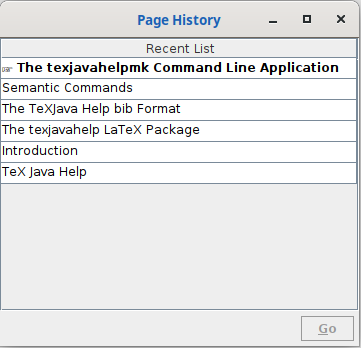
\includegraphics{images/historyframe}

\caption{The Page History Window}
\label{fig:historywindow}
\end{figure}

\menudef{menu.helpframe.navigation.historyback}

The \menu{helpframe.navigation.historyback} menu item, which is
also available as a button on the toolbar, will replace the current
view with the previously viewed page from this history list. The
item and button will be disabled if there is no previously viewed
page. 

\menudef{menu.helpframe.navigation.historyforward}

The \menu{helpframe.navigation.historyforward} menu item, which is
also available as a button on the toolbar, will replace the current view with the
next page in the history list. The item and button will be disabled if the
currently viewed page is at the end of the history list. 

\menudef*{menu.helpframe.settings}

The \menu{helpframe.settings} menu can be used to change the
graphical interface settings. These settings affect the primary and
secondary help windows, as well as some other related windows.
Note that this is separate from the main application settings.

\menudef{menu.helpframe.settings.decrease}

The \menu{helpframe.settings.decrease} item decreases the font
size by 1.

\menudef{menu.helpframe.settings.increase}

The \menu{helpframe.settings.increase} item increases the font
size by 1.

\menudef{menu.helpframe.settings.font}

The \menu{helpframe.settings.font} item opens the
\inlineglsdef{help_font_settings.title} dialog (see
\figureref{fig:helpfontdialog}). Use the
\widget{help_font_settings.family} selector for the main body font
family and the \widget{help_font_settings.size} selector for the
main body font size. Icon characters, such as
\gls{symbol.help.navigation.history.pointer}, may not be available
for your preferred font family, so you can specify an alternative
with the \widget{help_font_settings.icon_font_family} selector. This
will only list fonts that support some commonly used icon
characters.

\FloatFig
{fig:helpfontdialog}
{\includeimg
 [alt=
   {Help page font dialog}
 ]{images/helpfontdialog}%
}
{Help Page Font Dialog}

Use the \widget{help_font_settings.keystroke_font_family} selector to
choose the font to show keystrokes (such as
\keyref[textformat=keystrokefmt]{shift}) and the
\widget{help_font_settings.mono_font_family} selector to choose the
font to display code fragments (such as \verb|% \ { } #|).

\menudef{menu.helpframe.settings.nav}

The \menu{helpframe.settings.nav} item opens the
\inlineglsdef{help_settings_nav.title} dialog. This governs the
lower navigation bar (see \figureref{fig:helplowernavbar}) along the
bottom of the primary help window, which has smaller previous, up and next
buttons.  These buttons by default have the corresponding page
titles next to them, but they will be truncated if they exceed the
limit. This limit can be changed with the
\widget{help_settings_nav.label_limit} widget. Alternatively, you
can hide the text by deselecting the
\widget{help_settings_nav.show_label} checkbox.

\FloatFig
{fig:helplowernavbar}
{\includeimg
 [alt=
   {Help page lower navigation bar}
 ]{images/helplowernavbar}%
}
{Help Page Lower Navigation Bar}

\section{Secondary Help Window}
\label{sec:secondaryhelp}

The secondary help windows are more minimalist and will only show
the relevant \dgls{help-page} or set of pages that are applicable to the context
that was used to open the secondary help window. The search, history
and index items are unavailable. If only one page is applicable,
there won't be a navigation tree, otherwise the navigation tree will
only show the applicable pages.

\menudef*{menu.helpdialog.navigation}

The \menu{helpdialog.navigation} menu provides a way to move around
the topic pages.

\menudef{menu.helpdialog.navigation.reset}

The \menu{helpdialog.navigation.reset} item switches the current
page to the first page of the context topic.

\menudef{menu.helpdialog.navigation.historyback}

The \menu{helpdialog.navigation.historyback} goes back to the
previously visited page. Note that the history is specific to the
current secondary help dialog instance and does not include the history
from the primary help window.

\menudef{menu.helpdialog.navigation.historyforward}

The \menu{helpdialog.navigation.historyforward} moves forward in the
history list, if applicable.

\menudef{menu.helpdialog.navigation.previous}

The \menu{helpdialog.navigation.previous} menu item is only
available if there are multiple pages for the topic context and will
switch the current page with the previous page in the topic set.

\menudef{menu.helpdialog.navigation.up}

The \menu{helpdialog.navigation.up} menu item is only
available if there are multiple pages for the topic context and will
switch the current page with the parent page if it's within the topic set.

\menudef{menu.helpdialog.navigation.next}

The \menu{helpdialog.navigation.next} menu item is only
available if there are multiple pages for the topic context and will
switch the current page with the next page in the topic set.

\section{Image Viewer}
\label{sec:helpimageviewer}

The \menu{helppage.view_image} item in the \gls{index.menu.helppage} for both the
primary and secondary help windows will be enabled if the popup menu
is activated over an image. The \menu{helppage.view_image} item will
open the image in the \inlineglsdef{imageviewer.title} window.
If the image had alt text specified, this will be displayed in the
area above the image.

Within the \dialog{imageviewer} window, the image can be enlarged
using the \widget{imageviewer.magnify} spinner. The up and down
spinner controls go in steps of 25 (as opposed to the
\btn{menu.imageviewer.increase} and \btn{imageviewer.decrease}
action, which have an increment of 5). Alternatively, press the
shift key \keyref{shift} and drag the mouse to select an area to
zoom in on. Be sure to keep the shift key down when you release the
mouse. If you change your mind, release shift before releasing the
mouse button. If the shift key isn't pressed when you initiate the
drag, dragging will scroll the image instead. Double-clicking the
mouse on the image will go back to the previous magnification.

\menudef{index.menu.imageviewer}

The \gls{index.menu.imageviewer} is a popup menu that can
be activated anywhere over the image in the \dialog{imageviewer}
window. The following menu items are available.

\menudef{menu.imageviewer.fit_to_width}

The \menu{imageviewer.fit_to_width} item will scale the image so
that it fits the window width. This action has a corresponding
button on the toolbar.

\menudef{menu.imageviewer.fit_to_height}

The \menu{imageviewer.fit_to_height} item will scale the image so
that it fits the window height. This action has a corresponding
button on the toolbar.

\menudef{menu.imageviewer.fit_to_page}

The \menu{imageviewer.fit_to_page} item will scale the image so
that it fits within the window area. This action has a corresponding
button on the toolbar.

\menudef{menu.imageviewer.increase}

The \menu{imageviewer.increase} item will increase the current
magnification. This action has a corresponding
button on the toolbar.

\menudef{menu.imageviewer.decrease}

The \menu{imageviewer.decrease} item will decrease the current
magnification. This action has a corresponding
button on the toolbar.

\menudef{menu.imageviewer.zoom_1}

The \menu{imageviewer.zoom_1} item will set the magnification factor to
100\%. This action has a corresponding
button on the toolbar.

\menudef{menu.imageviewer.zoom_2}

The \menu{imageviewer.zoom_2} item will set the magnification factor to
200\%.

\menudef{menu.imageviewer.zoom_5}

The \menu{imageviewer.zoom_5} item will set the magnification factor to
500\%.

